\section{Positionsbestimmung}

\begin{frame}{Phasenverschiebung}
    \begin{columns}
        \begin{column}{0.5\textwidth}
            \begin{align}
                φ^\text{S}(t) &= f\cdot t-\frac{ρ}{\symup{c}}f+f\cdotδ^\text{S} \\
                φ_\text{E}(t) &= f\cdot t+f\cdotδ^\text{E} \\
                φ^\text{S}_\text{E} &= -\frac{ρ}{\symup{c}}f-f\cdot\incrementδ \\
                &= \incrementφ^\text{S}_\text{E}|^t_{t_0}+N \\
                N &= \text{\# empfangene Signale}
            \end{align}
        \end{column}
        \begin{column}{0.5\textwidth}
            \begin{figure}
                \centering
                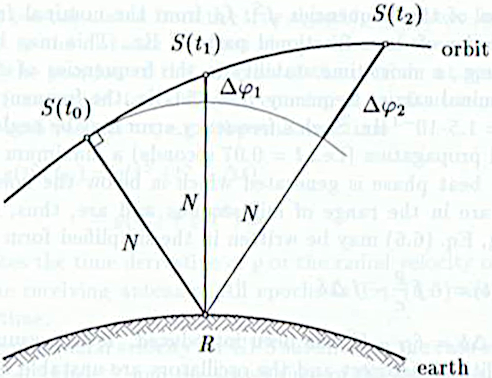
\includegraphics[width=\textwidth]{images/phasenverschiebung.jpg}
            \end{figure}
            \centering{\small[C,H-W,L]}
        \end{column}
    \end{columns}
\end{frame}

\begin{frame}{Zeitverzögerungen am Signal}
    S = Satellit, E = Empfänger
    \begin{align}
        t &= \text{Sende- /Empfangszeit} \\
        δ &= \text{zeitliche Verzögerungen, z.B. durch Rechenzeiten} \\
        t &= t(\text{GPS}) + δ
        \shortintertext{Zeitunterschied:}
        \increment t &= t_\text{E} - t^\text{S} = \increment t(\text{GPS}) +\incrementδ
        \shortintertext{Pseudoentfernung:}
        R &= \symup{c}\increment t = ρ + \symup{c}\incrementδ \label{eqn:pseudoentfernung}
        \shortintertext{Taylorreihe:}
        ρ\left(t_\text{E},\;t^\text{S}\right) &= ρ\left(t_\text{E},\;t^\text{S}+\increment t\right) = ρ\left(t^\text{S}\right)+\dot{ρ}\left(t^\text{S}\right)\cdot\increment t
        \shortintertext{Größe der ersten Korrektur:}
        \dot{ρ}\left(t^\text{S}\right)\cdot\increment t &\approx \SI{0.9}{\kilo\meter\per\second}\cdot\SI{0.07}{\second} =\SI{63}{\meter}
    \end{align}
\end{frame}

\begin{frame}{Ortskoordinaten}
    Man nimmt die Pseudoentfernung, Gleichung \eqref{eqn:pseudoentfernung}:
    \begin{align}
        R_\text{E}^\text{S}(t) &= ρ_\text{E}^\text{S}(t) + \symup{c}\incrementδ_\text{E}^\text{S}(t)
        \shortintertext{mit}
        ρ_\text{E}^\text{S}(t) &= \sqrt{\left(X^\text{S}(t)-X_\text{E}\right)^2+\left(Y^\text{S}(t)-Y_\text{E}\right)^2+\left(Z^\text{S}(t)-Z_\text{E}\right)^2}\;.
        \intertext{Der systematische Uhrenfehler wird angenähert}
        δ(t) &= a_0 + a_1(t-t_\text{r})+ a_2(t-t_\text{r})^2\;.
        \intertext{Es bleibt}
        R_\text{E}^\text{S}(t)& + \symup{c}δ^\text{S}(t) = ρ_\text{E}^\text{S}(t) + \symup{c}δ_\text{E}
    \end{align}
\end{frame}

\begin{frame}{Fehlerquellen}
    \begin{table}
        \centering
        \begin{tabular}{c c}
            \toprule
            {Fehlerquelle} & {Effekt} \\
            \midrule
            Signal    & Reflektionen in Atmosphäre und an Gebäuden \\
            Satellit  & falsche Orbitale \\
                      & Systematische Uhrfehler \\
            Empfänger & $^{\---}"^{\---}$ \\
                      & variable Emfängerfrequenz \\
            \bottomrule
        \end{tabular}
    \end{table}
\end{frame}
